\subsection{Circuito Derivador}



\subsection{Circuito Integrador}

\subsubsection{Introducción}

Se realizó el análisis de un circuito integrador ideal, utilizando en este caso tres componentes, una Resistencia $R$,
un capacitor $C$ y un amplificador operacional. 
Cabe destacar que se considera un integrador ideal ya que a diferencia del circuito RC analizado en el primer trabajo práctico de laboratorio,
éste funcionará como integrador para cualquier frecuencia y no solo a frecuencias altas. 

Los valores nominales utilizados para la experiencia fueron:

\begin{itemize}
	\item $R: 5.1K \Omega$ 
	\item $C: 20nF$
	\item $OPAMP: LM833$
\end{itemize}

\begin{figure}[H]
    \centering 
    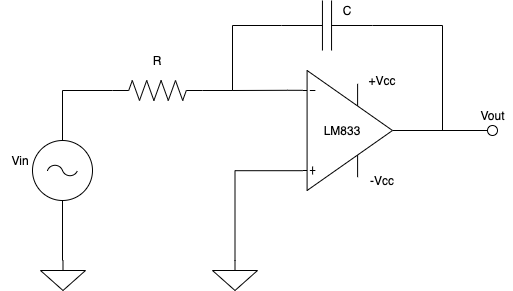
\includegraphics [scale=0.5] {../Ejercicio3-CircuitoIntegradoresyDerivadores/Imagenes/diagrama-integrador.png} 
    \caption{Diagrama del circuito integrador ideal empleado}
    \label{fig:emptyPlotTool}
\end{figure}

A continuación se procederá a calcular teóricamente el valor de las funciones transferencias para los casos en 
donde el amplificador operacional tiene un comportamiento ideal, con $A_{vol}$ finito y $A_{vol}(w)$ con polo dominante.

\subsubsection{Análisis de la Transferencia del Circuito Integrador - OPAMP ideal}

Para obtener la función transferencia en este caso, $H(S) = \frac{V_{out} (S)}{V_{in} (S)}$, partiremos de las siguientes condiciones
iniciales para el amplificador operacional:

\begin{itemize}
	\item $A_{vol}: \infty$
	\item $Z_{in}: \infty$
	\item $Z_{out}: 0$
\end{itemize}

\begin{figure}[H]
    \centering 
    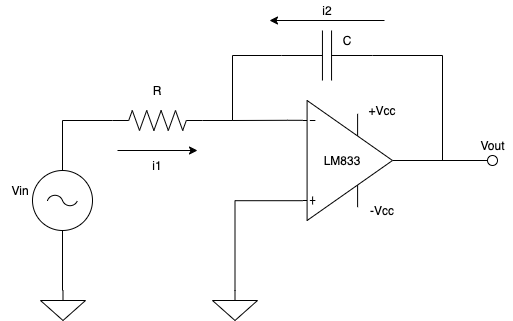
\includegraphics [scale=0.5] {../Ejercicio3-CircuitoIntegradoresyDerivadores/Imagenes/diagrama-integrador-corrientes.png} 
    \caption{Diagrama del circuito integrador ideal empleado}
    \label{fig:emptyPlotTool}
\end{figure}

Podemos observar a simple vista que:

\begin{itemize}
	\item $i1 = -i2$
	\item $i1 = \frac {V_{in}-V^{-}}{R} $
	\item $i2 = \frac {V_{out}-V^{-}}{X_c}$
	\item $V_{out} = A_{vol}(V^{+}-V^{-})$
\end{itemize}

Como ${A_{vol} \to \infty}$ y $V_{out}$ es finito, ${(V^{+}-V^{-}) \to 0}$ y como $V^{+}$ está conectado a tierra,
$(V^{-}$ representa tierra virtual, por lo cual su valor es de $0V$.

Entonces, redefiniendo las ecuaciones anteriores:

\begin{itemize}
	\item $i1 = \frac{V_{in}}{R} $
	\item $i2 = \frac {V_{out}}{X_c}$
\end{itemize}

Siendo entonces:

$$ \frac{V_{in}}{R} = - (\frac{V_{out}}{X_c}) \Longrightarrow \frac{V_{out}}{V_{in}} = -\frac{X_c}{R} = - \frac{1}{SRC}$$

$$ H(S) = - \frac{1}{SRC}$$

Claramente se puede apreciar que este circuito se comportará como un integrador, ya que si antitransformamos la función de transferencia
obtenida implicará que para obtener $v_{out}(t)$ habrá que integrar $v_{in}(t)$ en el dominio del tiempo. 

\subsubsection{Análisis de la Transferencia del Circuito Integrador - OPAMP con A finito}

A diferencia del caso anterior, aquí la diferencia en el cálculo de la función transferencia, $H(S) = \frac{V_{out} (S)}{V_{in} (S)}$,
entre el amplificador operaciones ideal y éste será:

\begin{itemize}
	\item $A_{vol}: finito$
\end{itemize}

Utilizando las mismas relaciones mencionadas en el apartado anterior, podemos observar ahora que:


$V_{out}=-A_{vol}.V^{-} \Longrightarrow V^{-} = \frac{-V_{out}}{A_{vol}}$ 


Por lo tanto:

\begin{itemize}
	\item $i1 = \frac {V_{in}-V^{-}}{R} =  \frac {V_{in} + \frac{V_{out}}{A_{vol}}}{R}$
	\item $i2 = \frac {V_{out}-V^{-}}{X_c} = \frac {V_{out} + \frac{V_{out}}{A_{vol}}}{X_c}$
\end{itemize}

Siendo entonces:

$$ \frac {V_{in} + \frac{V_{out}}{A_{vol}}}{R} = -(\frac {V_{out} + \frac{V_{out}}{A_{vol}}}{X_c})
\Longrightarrow \frac{V_{out}}{V_{in}} = \frac{1}{SCR(1+\frac{1}{A_{vol}}+\frac{1}{A_{vol}SRC})}$$

Finalmente:

$$H(S)= \frac{1}{SCR(1+\frac{1}{A_{vol}})+\frac{1}{A_{vol}}}$$

Es importante notar que siendo la ganancia para el caso ideal (GI) $- \frac{1}{SRC}$,  la funcion
transferencia se puede representar como $H(S) = GI. \frac{1}{SCR(1+\frac{1}{A_{vol}})+\frac{1}{A_{vol}}}$

\subsubsection{Análisis de la Transferencia del Circuito Integrador - OPAMP con $A_{vol}(w)$}

En este ultimo caso de analisis, $A_{vol}$ no es constante sino que es función de la frecuencia según:

$$A_{vol}=\frac{1}{1+\frac{S}{w_b}}$$

Por lo cual la expresion para la funcion transferencia calculada en el caso anterior, quedara denominada por:

$$H(S)= \frac{1}{SCR(1+\frac{1+\frac{1}{SCR}}{A_{vol}})}\Longrightarrow H(S)= \frac{1}{SCR(1+\frac{1+\frac{1}{SCR}}{\frac{1}{1+\frac{S}{w_b}}})}$$ 

Reacomodando algebraicamente:

$$H(S)=- \frac{1}{S^2\frac{W_b}{A_oCR}+SCR(1 + \frac{1}{A_o}+\frac{W_b}{CRA_o}) + \frac{1}{A_0}}$$

Podemos observar que si $A_o$ es muy grande, nuevamente estaremos en el caso donde la ganancia que obtendremos será la ideal para este circuito.

